\documentclass[9pt,twocolumn,twoside]{../../styles/osajnl}
\usepackage{fancyvrb}
\journal{i524} 

\title{Analysis Of People Relationship Using Word2Vec on Wiki Data}

\author[1,*]{Abhishek Gupta}
\author[1, **]{Avadhoot Agasti}

\affil[1]{School of Informatics and Computing, Bloomington, IN 47408, U.S.A.}

\affil[*]{Corresponding authors: abhigupt@iu.edu}
\affil[**]{Corresponding authors: aagasti@iu.edu}

\dates{project-1: Data mining for a wiki url , \today}

\ociscodes{Cloud, I524}

% replace this with your url in github/gitlab
\doi{\url{https://github.com/cloudmesh/sp17-i524/blob/master/project/S17-IR-P005/report/report.pdf}}

\begin{abstract}
Given a wiki URL of a person, find out his details like School, Spouse, Coaches, language, alma-meter etc Typically, the wiki page has all this information available but in the free form text. We need to converting it into structured data format so that it can help us analyze the people, from the networks etc We can create a network by navigating the people mentioned in the wiki page. 
\end{abstract}

\setboolean{displaycopyright}{true}


\begin{document}

\maketitle

\tableofcontents

\section{Introduction}

Use spark \cite{www-spark-python} to load the wiki data and create word vectors. Train it using spark ML  \cite{www-sparkml} and then use the model for analytics and prediction. The training set will use Word2Vec. Word2vec \cite{www-word2vec} is a group of related models that are used to produce word embeddings. Word2Vec is used to analyze the linguistic context of the words. In this project, we created Word2vec model using Wikipedia data. Our focus is people and organization names occurring in the Wikipedia data and to see if Word2vec can be used to understand relationship between people. Typically Wikipedia page for people and celebraties contain the entire family and friends, colleagues information. Our idea is to use Word2vec to see if using a smaller training set of known relationships whether we can derive similar relationship for anyone who has presence on Wikipedia. This mechanism can be then used to convert the data hidden in textual format to more structured data. 

\begin{center}
 \begin{tabular}{||c l||} 
 \hline
 Technology Name & Purpose  \\ [0.5ex] 
 \hline\hline
 spark \cite{www-spark-python} & data analysis  \\
 \hline
 sparkML \cite{www-sparkml} & machine learning  \\
 \hline
 python \cite{www-spark-python} & development \\
 \hline
 ansible \cite{www-ansible} & automated deployment \\
 \hline
 collectd \cite{www-collectd} & statistics collection for benchmarking \\
 \hline
\end{tabular}
\end{center}

\section{Plan}
Following table gives a breakdown of tasks in order to complete the project. Assuming week1 starts after submission of the proposal. These work items are high level breakdown on the tasks and may changes if needed.

\begin{center}
\begin{tabular}{ |c|l|c| } 
 \hline
Week & Work Item & Status \\
\hline
week1 & Basic POC of Word2Vec using Python  & planned \\ 
week2 & Scripts to download Wiki data & planned \\ 
week3 & Word2Vec Spark program & planned \\ 
week4 & Training and measuring accuracy & planned \\ 
week5 &  Ansible Deployment script for Spark & planned \\ 
week6 & Deployment and test on 2 clouds & planned \\ 
week7 & Performance measurement  & planned \\ 
week8 & Report Creation(parallel) & planned \\ 
 \hline
\end{tabular}
\end{center}

%\section{Design}
%TBD
\section{Design} \label{designsection}

\begin{figure}[htbp]
\centering
\fbox{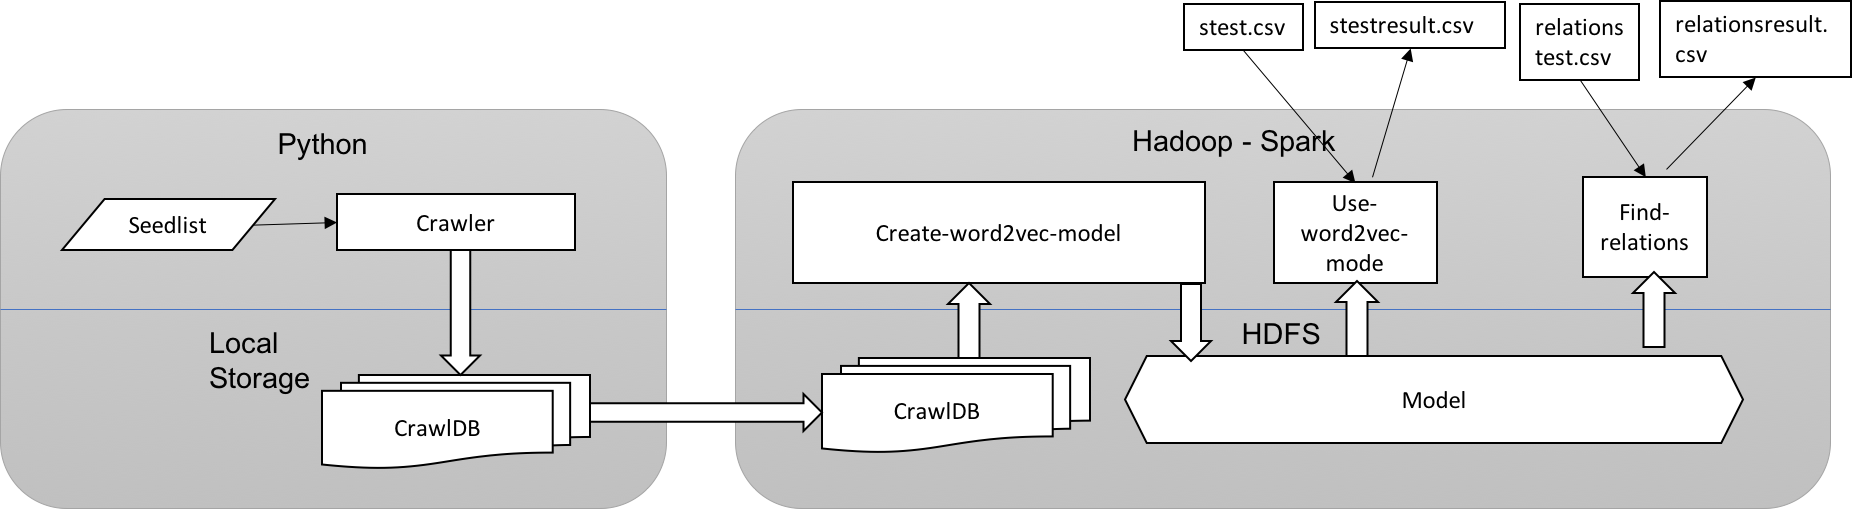
\includegraphics[width=\linewidth]{images/datapipeline.png}}
\caption{Data Pipeline.}
\label{fig:datapipeline}
\end{figure}

Figure \ref{fig:datapipeline} shows the overall data pipeline for the
project. The data pipeline has three important stages:
\begin{itemize}
\item Crawler: Crawler runs in batch mode on a standalone machine. It can
download wikipedia data as explained in section \ref{crawlersection}. Crawler
 creates CrawlDB which is a collection of text files. This crawler can be
 replaced or augmented with any web-crawler which can download or create the
 text files.

\item create-word2vec-model: This component is responsible for creating the
word2vec model for the text files in the CrawlDB. This model runs on Spark
and stores the model on HDFS. Section \ref{createmodelsection} describes this
 component in detail.

\item use-word2vec-model and find-relations: These two components use the
precreated word2vec model to find synonym of a word or find the relationships.
Section \ref{usemodel} describes these components in detail.
\end{itemize}

\subsection{Crawler} \label{crawlersection}
The Crawler component is useful to download the data from web. We implemented
 a simple crawler using Python which can deep traverse the wikipedia pages
 and download the text from it. In our crawler implementation, a user can
 specify the seed pages from wikipedia. User can also specify the maximum
 number of pages that are required to be downloaded. The crawler first
 downloads all the pages specified in the seedlist. It then extract the links
  from each wikipedia page and puts it in a queue which is internally
  maintained by the crawler. The crawler then downloads the the linked pages.
   Since this logic is implemented in recursive manner, the crawler can
   potentially download all the wikipedia pages which can be reached from the
   pages in the seedlist.

    We followed the seedlist based crawler approach so that we can retrieve
    domain specific web pages. A well chosen seedlist can fetch large number
    of relevant web pages.

 Figure \ref{fig:crawleralgo} is the flowchart of the crawler implementation.
\begin{figure}[htbp]
\centering
\fbox{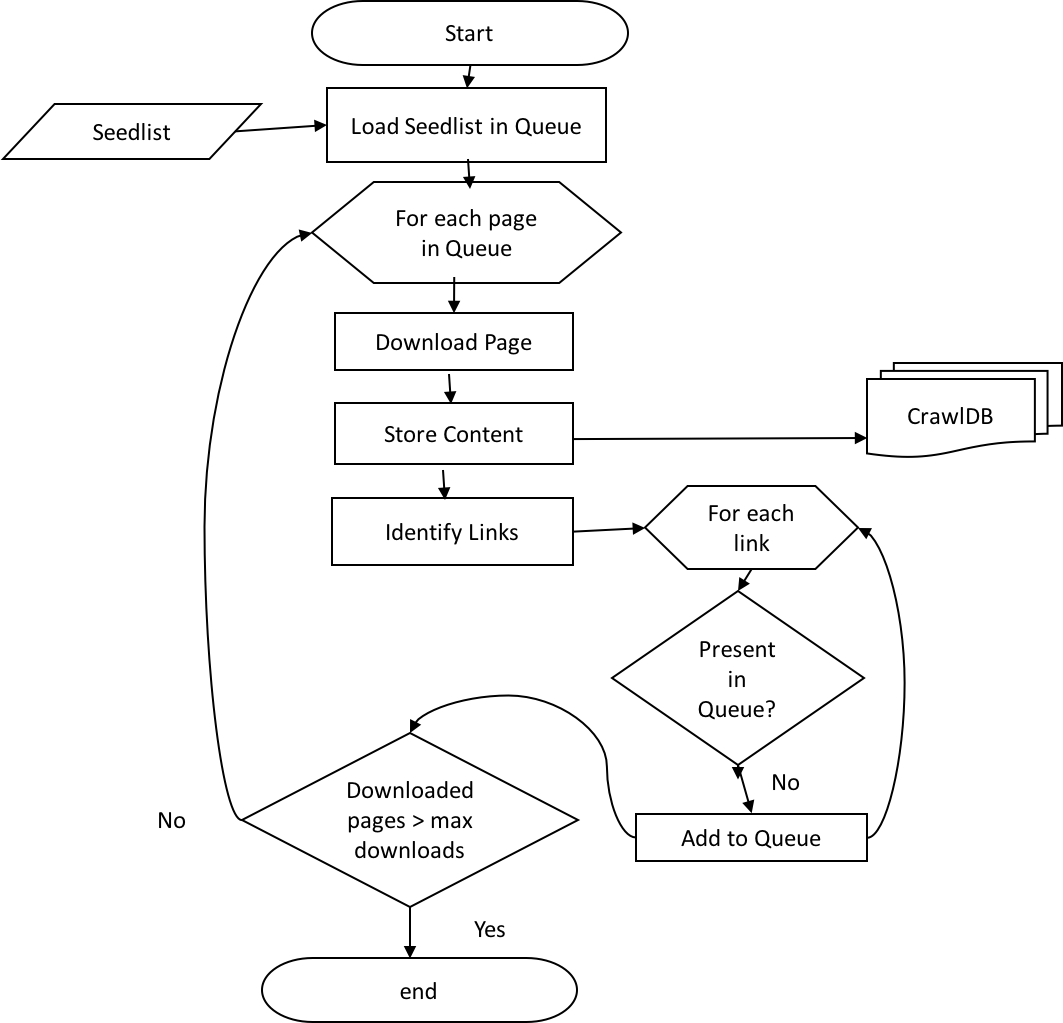
\includegraphics[width=\linewidth]{images/crawleralgo.png}}
\caption{Flowchart of crawler.}
\label{fig:crawleralgo}
\end{figure}

\subsection{Word2Vec Model Creation} \label{createmodelsection}


\subsection{Using the Word2Vec Model} \label{usemodel}




\section{Deployment} \label{deploymentsection}

The deployment on the cluster can be accomplished using 2 steps, assuming the cluster
is up and running
\begin{itemize}[noitemsep]
\item Step1: update hosts file \textit{ansible-word2vec/hosts} with the IP of the master. 
The first node on the cluster becomes the master node.
\item Step2: run the script  \textit{ansible-word2vec/run.sh}. This script will run the ansible 
playbooks to accomplish stage1 through stage4 of the deployment process.
\end{itemize}

\begin{figure}[htbp]
\centering
\fbox{\includegraphics[width=\linewidth]{images/deployment.png}}
\caption{Deployment stages.}
\label{fig:deploymentstages}
\end{figure}

Figure \ref{fig:deploymentstages} shows the deployment stages. The two steps
accomplish deployment in multiple stages as discussed in the sections below.

\subsection{Stage1} \label{deploymentstage1} 
As pre-requisite, we need to create a cluster with 1 or more nodes.
We created a 3 node cluster using Cloudmesh \cite{www-cloudmesh} command line interface(CLI). 
Cloudmesh\cite{www-cloudmesh} CLI allows you to orchestrate virtual machines(VM) in a 
cloud environment. For this project, we have used Chameleon and Jetstream cloud 
providers to orchestrate the VMs using cloudmesh\cite{www-cloudmesh} CLI. We can orchestrate a 3 node 
cluster using following CLI:

\begin{verbatim}
cm reset
pip uninstall cloudmesh_client
pip install -U cloudmesh_client
cm key add --ssh
cm refresh on
cm cluster define --count 3 \
	--image CC-Ubuntu14.04 --flavor m1.medium
cm hadoop define spark pig
cm hadoop sync
cm hadoop deploy
cm cluster cross_ssh
\end{verbatim}   

We are using Ubuntu14.04 image with m1.medium which comes with 2 CPU, 4GB
memory. Also, the nodes created are having hadoop and spark add-ons.
We can test the deployment by checking hdfs and spark-submit CLI work fine.
\begin{verbatim}
ssh cc@<cluster-ip>
sudo su - hadoop
hdfs
spark-submit
\end{verbatim}

At this stage our cluster is ready for further deployments.

\subsection{Stage2} \label{deploymentstage2}  
By default, cloudmesh installs spark 1.6 but our word2vec solution requires
spark 2.1. We need to upgrade spark on the cluster. In order to do so we can run 
\textit{install\_upgrade\_spark.yaml} ansible\cite{www-ansible} playbook. This will download and unpack spark2.1 
tar ball and further update the softlink to point to spark 2.1 folder.

\subsection{Stage3} \label{deploymentstage3} 
In this step, we upgrade the development libraries for python, and pip,
install python modules like wkipedia, request etc, download the code from git repo and
install it in \textit{/opt/word2vec} folder, set the folder permissions for the \textit{/opt/word2vec} folder
so that it can be executed by hadoop user. These steps can be achieved using 
\textit{word2vec\_setup.yaml} playbook. After completing this stage, we are ready for running
our word2vec solution on the cluster. 

\subsection{Stage4} \label{deploymentstage4} 
This stage primarily deals with submitting the jobs for various purpose. 
Before we submit the jobs, we need to make sure input folder are created on hadfs.
First, we run the crawler to download the training set and upload the data on hdfs.
Further we run various jobs to created model and find relations. Along with these jobs
we also run some monitoring jobs. The monitoring job queries spark metrics using 
\begin{verbatim}
http://${spark_master}:4040
\end{verbatim}

Stage4 steps can be accomplished using \textit{word2vec\_execute.yaml} playbook. 

At the end of stage4 we also fetch the execution results from the cluster along with the 
metrics of execution times at various stages. The output files are fetched into \textit{/tmp/word2vec\_results}
\begin{verbatim}
ls -1t /tmp/word2vec_results
jobs.csv
executors.csv
app.csv
stest.csv
relationstest.csv
stestresult.csv
relationsresult.csv
\end{verbatim}
Files \textit{jobs.csv, executors.csv, and app.csv} collect the execution time for various jobs. 
File \textit{relationsresult.csv} file collects the results for sample relations corresponding to
\textit{relationstest.csv}. Similarly \textit{stestresult.csv} collects the results corresponding to \textit{stest.csv}.

\subsection{Execution} \label{deploymentexecution}
\subsubsection{Cleanup}
We can execute the run from local system using  \textit{run.sh} located inside \textit{ansible-word2vec}. 
Run script executes all stages sequentially on the remote system. To rerun word2vec, run the cleanup 
playbook \textit{word2vec\_cleanup.yaml} located inside \textit{ansible-word2vec}.  Cleanup remove 
the spark 2.1 binary and the soft link, remove \textit{/opt/word2vec} folder as well as any temporary files created
during setup step.

\subsubsection{Page size}
The crawler downloads pages from wikipedia based on the config page count. To modify the page count, 
we can edit \textit{ansible-word2vec/setupvariables.yml} and set the \textit{max\_pages} to desired 
page size. The crawler downloads individual pages and then combines the pages into a single file
before submitting the spark jobs.

\subsubsection{Test Results}
Test results are downloaded to local machine in  \textit{/tmp/word2vec\_results} folder. Ansible execution
log is saved in \textit{/tmp/word2vec-logfile.txt}. The log gets appended each time you execute the run 
script.

\subsubsection{Troubleshooting}
\begin{enumerate}
\item If the installation \textit{run.sh} script fails in middle due to some reason, execute the cleanup script
before re-triggering run script again. The run script may fail due to variety of reasons like failed to shh,
hadoop not available etc
\item If the run script fails due to spark memory errors, you can modify the spark memory setting in
 \textit{code/config.properties} push the code to a git feature branch for example spark\_test. Modify
 \textit{word2vec\_setup.yaml} git section \textit{version=master} to point to spark\_test branch and 
 execute the run script.
 \item If hadoop goes into safe mode, goto the cluster namenode and execute the following
 \begin{verbatim}
 /opt/hadoop$ bin/hadoop dfsadmin -safemode leave
 \end{verbatim}
 This will remove the cluster from safe mode.
 \end{enumerate}
 
 
 



\section{Benchmarking}
Solution will use collectd \cite{www-collectd} to collect statistics. Once the solution is deployed to the cluster. We should benchmark parameters like
\begin{itemize}[noitemsep]
\item cpu
\item memory
\item throughput reads/writes
\end{itemize}
Benchmarking will be done for one or more cloud providers. The deployment scripts should be agnostic to the cloud provider. 

\section{Discussion}
TBD

\section{Conclusion}

Using this wiki analysis we should be able to build a network based on wiki data.

\section{Acknowledgement}

We acknowledge our professor Gregor von Laszewski and all associate instructors for helping us and guiding us throughout this project.

\section{Appendices}
TBD

% Bibliography

\bibliography{references}
 

\end{document}
